% !TEX root = MusicFormatsUserGuide.tex

% -------------------------------------------------------------------------
\chapter{MFSL (MusicFormats Scripting Language}
% -------------------------------------------------------------------------

\mfslLang\ is meant for launching \mf\ tools easily, gathering options for them and providing selection criteria to do so. The syntax and semantics are very simple, for use by musicians.

A file containing \mfslLang\ elements is called a {\it \script}, with name extension \code{.mfsl} typically, though other extensions can be used at will.

The main features of \mfslLang\ are:
\begin{itemize}
\item the options are written the same as in OAH, such as \code {-global-staff-size 25.5};

\item the numbers and strings in options values are written the same as in OAH too -- 'a single quotes string', "a double quotes string";

\item a small number of names are reserved keywords:
\begin{itemize}
\item \code{tool}, to specify the \mf\ \tool\ to be run;
\item \code{input}, to indicate the input source when the \tool\ is launched, a file name or \code{-} for \standardInput;
\item \code{choice}, \code{default} and \code{case}, to \select\ options or others depending on the needs;
\item \code{select} and \code{all}, to indicate whether the tool should be launched once or multiple times;
\item comments can be used in \script s: they can be span from a \code{\#} to the end of the line, or span multiple lines, starting and ending with \code{\#\#\#}.
\end{itemize}
\end{itemize}

The names in a \choice\ specification are so-called \MainIt{labels}, here "tutti", "soprano", alto", "tenor" and "bass":
\begin{lstlisting}[language=MFSL]
choice SCORE :
  tutti | soprano | alto | tenor | bass,

  default: tutti
;
\end{lstlisting}

An \MainIt{interpreter} maned \mfslExec\ is provided by \mf\, that can run \mfslLang\ \script s as is done by the usual shells and languages such as Python or Ruby:
\begin{lstlisting}[language=Terminal]
jacquesmenu@macmini > mfsl -about
What mfsl does:

    This interpreter reads text input containing
    a tool name, an input source name, keywords and options,
    and launches the specified tool
    with these options applied to the input source name.

    The input can come from a file or from standard input,
    allowing the interpreter to be used interactively or in shell pipes.

    The activity log and warning/error messages go to standard error.
\end{lstlisting}

This chapter first presents \mfslLang\ with example scripts, and then the MFSL language in a more formal way.


% -------------------------------------------------------------------------
\section{A MusicXML example}
% -------------------------------------------------------------------------

We use the \mfslfiles{Hymn121.xml} \mxml\ file in this chapter to show more and more useful uses of the \mfslInterp.

The score used as a starting point is:\\
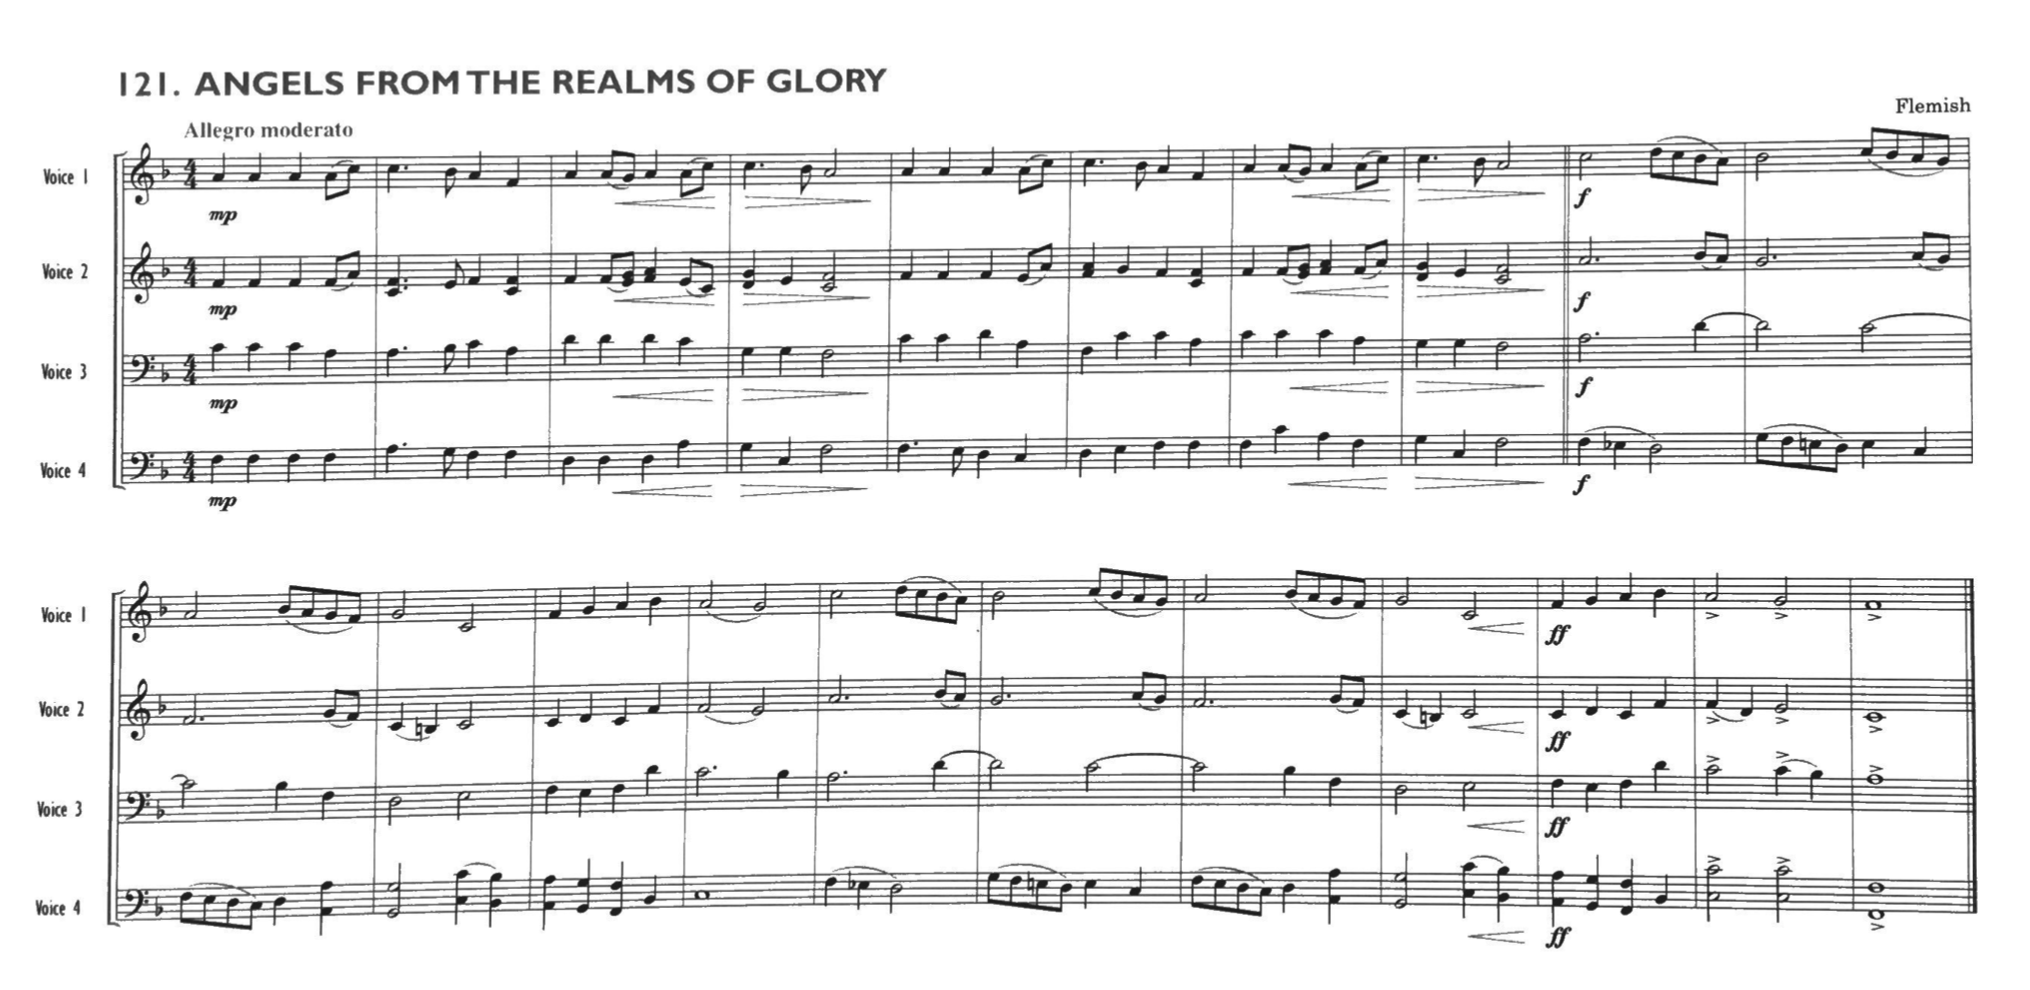
\includegraphics[scale=0.5]{../graphics/Hymn121_OrigianlScore.png}

From that:
\begin{itemize}
\item the original PDF file has been scanned with \Main{Photo Score Ultimate\texttrademark} to obtain\\
 \mfslfiles{Hymn121.xml}

\item a glitch has been introduced in the last measure of part \code{P4} in the form of a \musicXmlMarkup{lyric} element:
\begin{lstlisting}[language=MusicXML]
    <lyric number="1">
     <syllabic>begin</syllabic>
     <text>glitch</text>
    </lyric>
\end{lstlisting}
\end{itemize}


% -------------------------------------------------------------------------
\section{A first, minimal MFSL script example}
% -------------------------------------------------------------------------

The \mfslfiles{minimal.mfsl} \script\ illustrates two basic features of \mfslLang:
\begin{lstlisting}[language=MFSL]
jacquesmenu@macmini: ~/musicformats-git-dev/mfslfiles > cat minimal.mfsl
#!/Users/jacquesmenu/musicformats-git-dev/build/bin/mfsl

# This is a comment (for human readers), from '#' to the end of line

# The first line above contains a so-called shebang,
# a special comment indicating the access path to the MFSL interpreter
# used to process the remainder of this file

###
  And here is a multi-line comment.

  This minimal MFSL script contains only the mandatory elements:
    - a tool specification, telling which MusicFormats tool to use,
      here xml2ly;

    - an input specification, specifying the input source for this tool,
      here file name "Hymn121.xml".

      It can be a file name or '-' to specify standard input.

      Typing './minimal.mfsl' in a terminal causes xml2ly to be launched,
      in a way equivalent to the direct command:
          mxl2ly Hymn121.xml

      Useful scripts contain options in complement to that,
      since MFSL is intended to gather options to be used by the tool.
###


# ----------------------------------------------------------
# the MusicFormats tool to be used
# ----------------------------------------------------------

tool : xml2ly ;


# ----------------------------------------------------------
# the input file to be processed by the tool
# ----------------------------------------------------------

input : "Hymn121.xml" ;

# double quote can be used also to delimitate strings:
# input : 'Hymn121.xml'

# this would be OK too, since there are no spaces in the file name
# input : Hymn121.xml
\end{lstlisting}


% -------------------------------------------------------------------------
\section{Launching an MFSL script}
% -------------------------------------------------------------------------

This first line of an \mfslLang\ \script\ is the so-called \MainIt{shebang}. It contains the \filePath\ to the \mfslInterp, allowing running such a \script by its name from the terminal, provided the \script\ file is made executable.

This can be done in the \OS\ file system \GUI, or using the \code{chmod} command or equivalent in a terminal:
\begin{lstlisting}[language=Terminal]
jacquesmenu@macmini: ~/musicformats-git-dev/mfslfiles > chmod +x minimal.mfsl

jacquesmenu@macmini: ~/musicformats-git-dev/mfslfiles > ls -sal minimal.mfsl
8 -rwxr-xr-x@ 1 jacquesmenu  staff  1488 Mar 26 18:20 minimal.mfsl
\end{lstlisting}

The \mfslInterp\ has the \optionNameBoth{no-launch}{nol} option to display the essential information found in the script and quit without actually running the tool:
\begin{lstlisting}[language=Terminal]
jacquesmenu@macmini: ~/musicformats-git-dev/mfslfiles > mfsl -query no-launch
--- Help for atom "no-launch" in subgroup "MFSL"
    -no-launch, -nol
          Analyze the MFSL script, but don't launch the tool actually.
          This is useful to check the options gathered by the MFSL interpreter,
          and what command(s) would be launched.
          This option implies the '-display-tool-and-input, -ttai' option.
jacquesmenu@macmini: ~/musicformats-git-dev/mfslfiles >
\end{lstlisting}

The \optionNameBoth{display-tool-and-input}{dtai} option itself has this effect:
\begin{lstlisting}[language=Terminal]
jacquesmenu@macmini: ~/musicformats-git-dev/mfslfiles > mfsl -query display-tool-and-input
--- Help for atom "display-tool-and-input" in subgroup "MFSL"
    -display-tool-and-input, -dtai
          Write MFSL tool and input analysis activity to standard output.
\end{lstlisting}

When running the \mfslfiles{minimal.mfsl} \script\ from the \CLI\ with \optionBoth{no-launch}{nol}, we get:
\begin{lstlisting}[language=Terminal]
jacquesmenu@macmini: ~/musicformats-git-dev/mfslfiles > ./minimal.mfsl -no-launch
====> The known tools names are: ["msdlconverter", "xml2brl", "xml2gmn", "xml2ly" and "xml2xml"]
====> tool: xml2ly
====> input: Hymn121.xml
====> Launching xml2ly with the argument and option gathered from ./minimal.mfsl
====> The command to be executed is:
  xml2ly Hymn121.xml
====> The command above is *NOT* executed
\end{lstlisting}

Launching it without this options gives the following. The output of the \mfslInterp\ goes to standard output by defaut, so we redirect that to file \mfslfiles{Minimal.ly}:
\begin{lstlisting}[language=Terminal]
jacquesmenu@macmini: ~/musicformats-git-dev/mfslfiles > ./minimal.mfsl > Minimal.ly

jacquesmenu@macmini: ~/musicformats-git-dev/mfslfiles > ls -sal Minimal.ly
24 -rw-r--r--  1 jacquesmenu  staff  11772 Mar 28 09:44 Minimal.ly
\end{lstlisting}

The score can then be obtained with LilyPond from \mfslfiles{Minimal.ly}. It is shown at \FigureRef{The score created with minimal.mfsl}.
\begin{figure}[p]
\begin{center}
\caption {The score created with {\tt minimal.mfsl}}
\label{The score created with minimal.mfsl}

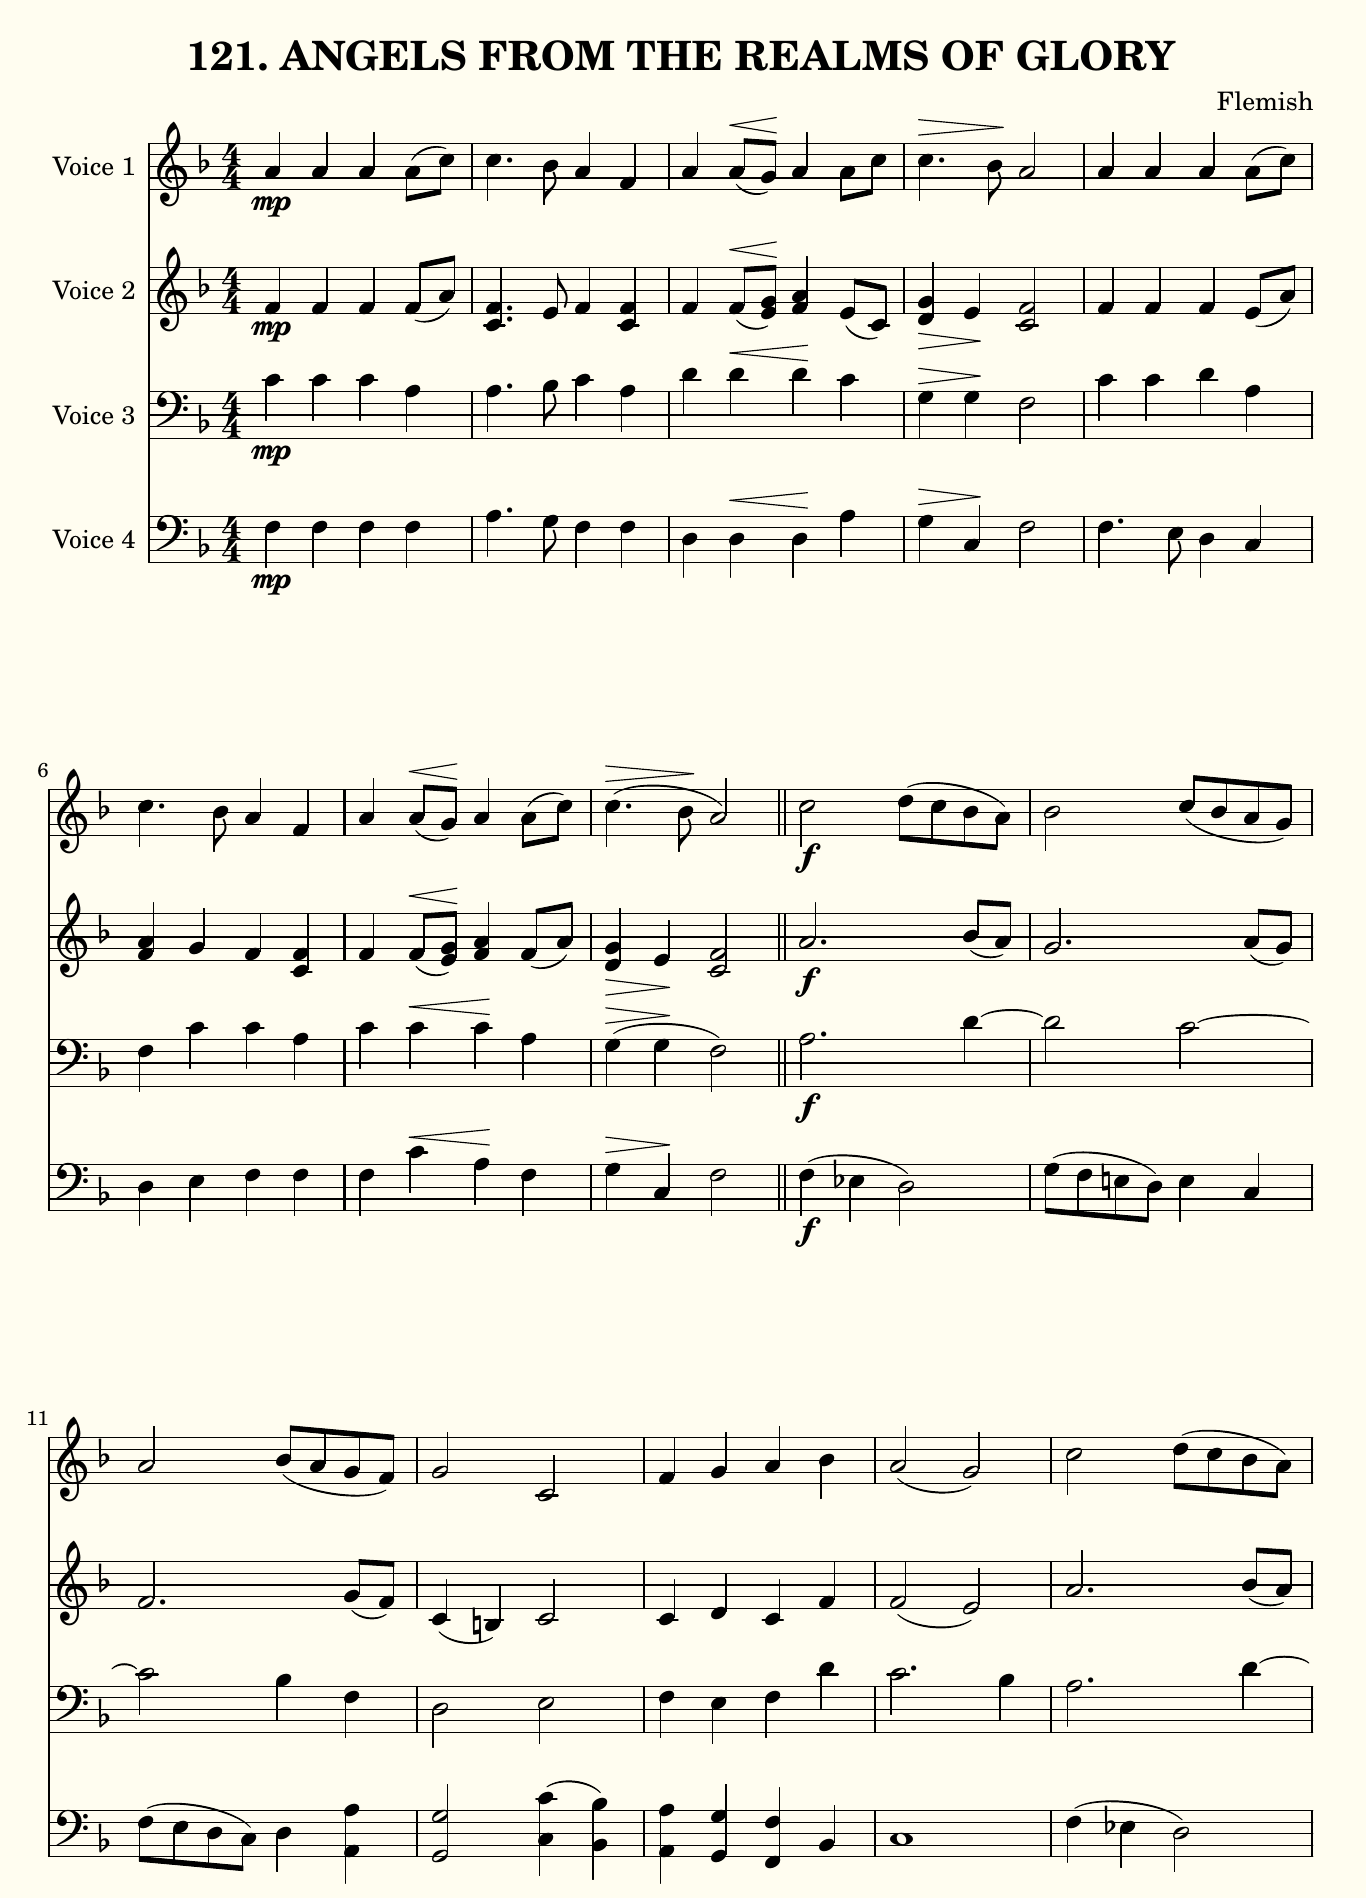
\includegraphics[scale=0.5]{../graphics/Minimal_page1.png}
%\vspace{4cm}
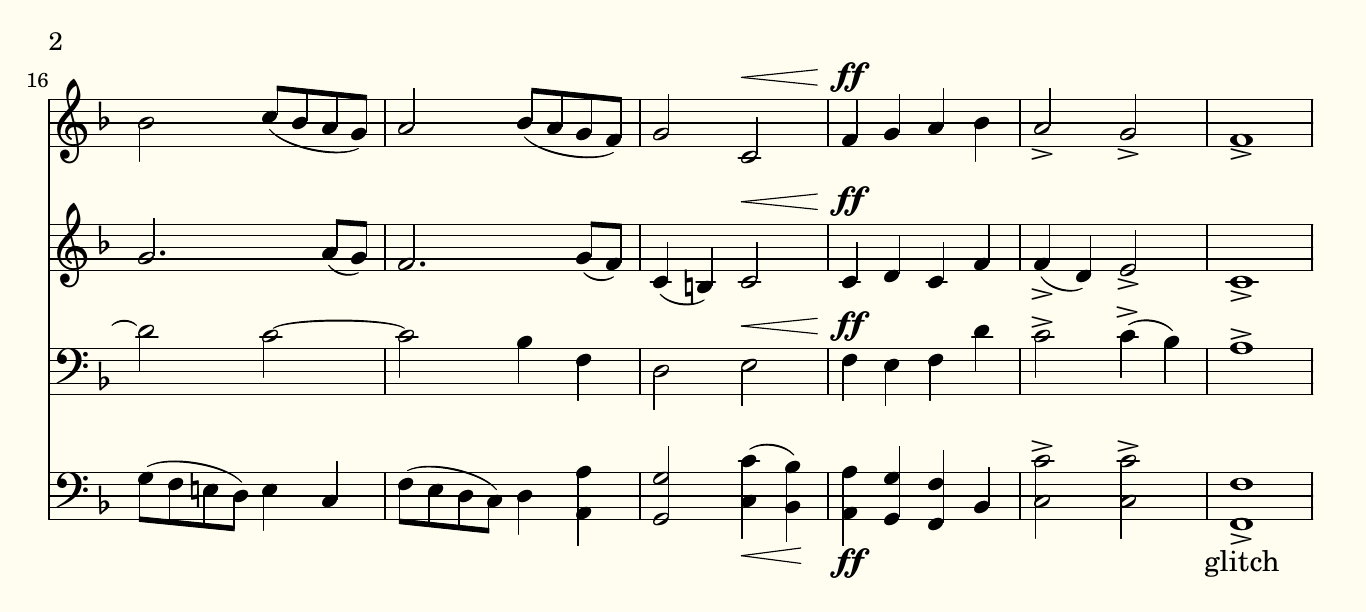
\includegraphics[scale=0.5]{../graphics/Minimal_page2.png}

\end{center}
\end{figure}


% -------------------------------------------------------------------------
\section{Interactive use of the MFSL interpreter}
% -------------------------------------------------------------------------

As is traditional when using interpreters from the \CLI, the \mfslInterp\ \mfslExec\ can be launched without any file name or with a '\code{-}' denoting \standardInput.

If that is done in a terminal, a \code{Ctrl-d} (control key held when typing the {\tt d}) should be typed after the input, to indicate the end of it, such as:
\begin{lstlisting}[language=Terminal]
jacquesmenu@macmini: ~/musicformats-git-dev/mfslfiles > mfsl
tool : xml2ly ;
input : "HelloWorld.xml" ;

-auto-output-file-name
-display-cpu-usage
							===> Ctrl-d typed here to indicate the end of input
Timing information:

Activity  Description                                             Kind       CPU (sec)
--------  ------------------------------------------------------  ---------  ---------

          Handle the options and arguments from argc/argv         mandatory    0.03659
Pass 1    Create an MXSR reading a MusicXML file                  mandatory    0.00336
Pass 2a   Create an MSR skeleton from the MXSR                    mandatory    0.00157
Pass 2b   Populate the MSR skeleton from MusicXML data            mandatory    0.00199
Pass 3    Convert the first MSR into a second MSR                 mandatory    0.00059
Pass 4    Convert the second MSR into an LPSR                     mandatory    0.00065
Pass 5    Convert the LPSR score to LilyPond code                 mandatory    0.00111

Total (sec)  Mandatory  Optional
-----------  ---------  ---------
0.04586      0.04586    0.00000

jacquesmenu@macmini: ~/musicformats-git-dev/mfslfiles > ls -sal HelloWorld.ly
8 -rw-r--r--@ 1 jacquesmenu  staff  1221 Mar 28 07:48 HelloWorld.ly
\end{lstlisting}


% -------------------------------------------------------------------------
\section{The structure of MFSL scripts}
% -------------------------------------------------------------------------

\mfslLang\ is about collecting options to launch a \mf\ tool using some specified input.

Thus, an \mfslLang\ \script\ starts by:
\begin{itemize}
\item a mandatory \code{tool} specification: it tells which MusicFormats tool
    to use, here \xmlToLy;

\item  a mandatory  \code{input} specification: it tells the input source to apply
    the tool to, such as \fileName{Hymn121.xml} above.
\end{itemize}

After that, there can be:
\begin{itemize}
\item  any number of MusicFormats options;

\item  any number of  \code{choice} specifications identified by so-called \MainIt{labels}, to provide options selection criteria;

\item any number of  \code{case} statements stating the options to be used depending on
  the selected \choice\ labels;

\item optionaly, any number of \code{select} statements.

\end{itemize}

The details are presented in the forthcoming sections.


% -------------------------------------------------------------------------
\section{Options to the MFSL interpreter}
% -------------------------------------------------------------------------

The \mfslInterp\ has its own options, which can be displayed by \optionBoth{help}{h}.

The specific options are placed in two groups. The first one, seen with \optionBoth{help-user}{hu}, is for regular users:
\begin{lstlisting}[language=Terminal]
jacquesmenu@macmini: ~/musicformats-git-dev/mfslfiles > mfsl -help-user
--- Help for subgroup "MFSL" in group "MFSL group" ---
  MFSL group (-help-mfsl-user-group, -hmfsl-user-group):
  --------------------------
    MFSL (-help-user, -hu):
      -display-tokens, -dtoks
            Write a trace of the MFSL tokens to standard error.
      -display-tool-and-input, -dtai
            Write MFSL tool and input analysis activity to standard output.
      -display-options, -dopts
            Write MFSL options analysis activity to standard output.
      -select, -sel CHOICE:LABEL
            Select LABEL for choice CHOICE.
            The tool will be run once using the corresponding options block(s).
      -all CHOICE
            Select each label for choice CHOICE in turn.
            The tool will be run as many times, using the corresponding options block(s).
      -no-launch, -nol
            Analyze the MFSL script, but don't launch the tool actually.
            This is useful to check the options collected by the MFSL interpreter,
            and what command(s) would be launched.
            This option implies the '-display-tool-and-input, -ttai' option.
\end{lstlisting}

The second group, diplayed by \optionBoth{help-maintainer}{hm}, if for the curious and the maintainers of \mf:
\begin{lstlisting}[language=Terminal]
jacquesmenu@macmini: ~/musicformats-git-dev/mfslfiles > mfsl -help-maintainer
--- Help for subgroup "MFSL" in group "MFSL group" ---
  MFSL group (-help-mfsl-maintainance-group, -hmfsl--maintainance-group):
  --------------------------
    MFSL (-help-maintainer, -hm):
      -trace-scanning, -tscan
            Write a trace of the MFSL scanning by Flex-generated code to standard error.
      -trace-parsing, -tparse
            Write a trace of the MFSL parsing by Bison-generated code to standard error.
      -trace-choices, -tchoices
            Write MFSL choice analysis activity to standard output.
      -trace-choice-statements, -tchoicesstats
            Write MFSL choice statements handling activity to standard output.
      -trace-case-input-statements, -tinputs
            Write MFSL case statements handling activity to standard output.
      -trace-case-choice-statements, -tcasechoices
            Write MFSL case statements handling activity to standard output.
      -trace-options-blocks, -toblocks
            Write MFSL options blocks analysis activity to standard output.
\end{lstlisting}


% -------------------------------------------------------------------------
\section{Options in an MFSL script body}
% -------------------------------------------------------------------------

The \mxml\ file \mfslfiles{Hymn121.xml} contains four parts, named \code{P1} to \code{P4}.

Let us now use options to produce a bass score from this file. This is done by:
\begin{itemize}
\item  filtering the \mxml\ data to keep only part \code{P4};
\item  using options to obtain the desired result.
\end{itemize}

The \mfslfiles{Hymn121ForBass.mfsl} script contains enhancement options that we will keep commented for the time being:
\begin{lstlisting}[language=MFSL]
jacquesmenu@macmini: ~/musicformats-git-dev/mfslfiles > cat Hymn121ForBass.mfsl
#!//Users/jacquesmenu/musicformats-git-dev/build/bin/mfsl

###
  This MFSL script contain s:
    - a 'tool' specification, telling which MusicFormats tool
      to use, here xml2ly;

    - an 'input' specification, the input source to apply
      the latter to, here file name "Hymn121.xml";

    - a number of MusicFormats options,
      which can easily be commented/uncommented at will.
###


# ----------------------------------------------------------
# the MusicFormats tool to be used
# ----------------------------------------------------------

tool : xml2ly ;


# ----------------------------------------------------------
# the input file to be handled by the tool
# ----------------------------------------------------------

input : "Hymn121.xml" ;


# ----------------------------------------------------------
# basic options
# ----------------------------------------------------------

# output
  -output-file-name "Hymn121_Bass.ly"

# header
  -title "Hymn 121 - Angels From The Realms Of Glory"
  -subtitle "Part 4 - Bass"

  -keep-musicxml-part-id P4

# display
 -display-options-values
#  -display-msr-1-short
#  -display-lpsr-short

# LilyPond
  -lilypond-generation-infos


# ----------------------------------------------------------
# enhancement options
# ----------------------------------------------------------

# staff
#   -lpsr-staff-instrument-name "Voice 4:"  # an empty name

# dynamics
#   -all-wedges-below   # there are above the staff in the input file

#   -ignore-musicxml-lyrics
#      # there's a glitch in the last measure of the bass...
\end{lstlisting}

Let us run this script with:
\begin{lstlisting}[language=Terminal]
jacquesmenu@macmini: ~/musicformats-git-dev/mfslfiles > ./Hymn121ForBass.mfsl
  The options values for xml2ly are:
    Files group (-help-files-group, -hfiles-group), 1 atom chosen:
    --------------------------
      Files (-help-files, -hfiles), 1 atom chosen:
        fOutputFileName                                 : [Hymn121_Bass.ly], set by user

    Options and help group (-help-oah-group, -hoah-group), 1 atom chosen:
    --------------------------
      Options and help (-help-oah, -hoah), 1 atom chosen:
        fDisplayOptionsValues                           : true, set by user

    Parts group (-help-parts-group, -hparts-group), 1 atom chosen:
    --------------------------
      Parts (-help-parts, -hparts), 1 atom chosen:
        fMusicXMLPartsKeepIDSet                         : set by user
          "P4"

    Header group (-help-header-group, -hheader-group), 2 atoms chosen:
    --------------------------
      Header (-help-header, -hheader), 2 atoms chosen:
        fTitle                                          : [Hymn 121 - Angels From The Realms Of Glory], set by user
        fSubTitle                                       : [Part 4 - Bass], set by user

    Output group (-help-output-group, -houtput-group), 1 atom chosen:
    --------------------------
      Output (-help-output, -houtput), 1 atom chosen:
        fXml2lyInfos                                    : true, set by user

jacquesmenu@macmini: ~/musicformats-git-dev/mfslfiles > ls -sal Hymn121_Bass.ly
16 -rw-r--r--@ 1 jacquesmenu  staff  4586 Apr  5 11:18 Hymn121_Bass.ly
\end{lstlisting}

The score we obtain is:\\
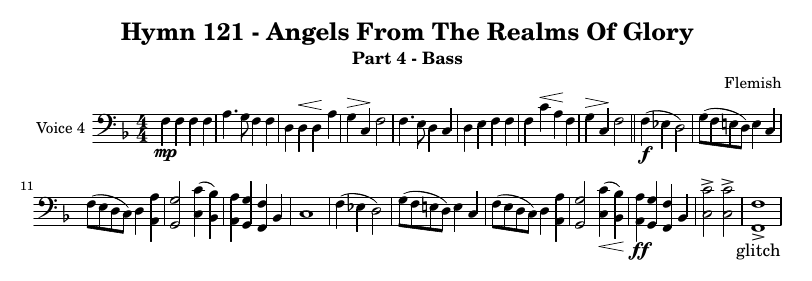
\includegraphics[scale=0.8]{../graphics/Hymn121_Bass.png}


% -------------------------------------------------------------------------
\section{Enhancing the produced score}
% -------------------------------------------------------------------------

The score obtained above is imperfect, but \xmlToLy\ has options that can help us:
\begin{itemize}
\item the instrument name 'Voice 4' is not relevant for this single-voice score.

		This can be replaced by an empty name with:
\begin{lstlisting}[language=Terminal]
jacquesmenu@macmini > xml2ly -query lpsr-staff-instrument-name
--- Help for atom "lpsr-staff-instrument-name" in subgroup "Staves"
    -lpsr-staff-instrument-name, -lpstaffinstrname STAFF_INSTRUMENT_NAME_SPEC
          STAFF_INSTRUMENT_NAME_SPEC should be of the form STAFF:NAME.
          Set the instrument name of staff STAFF to NAME, for example after displaying
          the names in the score or a summary of the latter in a first run with options
          '-display-msr-names, -dmsrnames' or '-display-msr-summary, -dmsrsum'.
          There can be spaces around the ':', in which case quoting is needed.
          There can be several occurrences of this option.
\end{lstlisting}

\item the dynamic wedges $<$ and $>$ are placed above the staff.

	This can be fixed with:
\begin{lstlisting}[language=Terminal]
jacquesmenu@macmini > xml2ly -query all-wedges-below
--- Help for atom "all-wedges-below" in subgroup "Wedges"
    -all-wedges-below, -awb
          Ignore wedges placement and set it to 'below'.
\end{lstlisting}

\item there is the lyrics glitch at the end of the bass part.

The \musicXmlMarkup{lyric} element can be ignored with this option:
\begin{lstlisting}[language=Terminal]
jacquesmenu@macmini > xml2ly -query ignore-musicxml-lyrics
--- Help for atom "ignore-musicxml-lyrics" in subgroup "Lyrics"
    -ignore-musicxml-lyrics, -imlyrics
          Ignore lyrics in MusicXML data.
\end{lstlisting}
\end{itemize}

These options can be applied by uncommenting them in \mfslfiles{Hymn121ForBass.mfsl}. The differences between the two are:
\begin{lstlisting}[language=Terminal]
jacquesmenu@macmini: ~/musicformats-git-dev/mfslfiles > diff Hymn121ForBass.mfsl Hymn121ForBassEnhanced.mfsl
35c35
<   -output-file-name "Hymn121_Bass.ly"
---
>   -output-file-name "Hymn121_BassEnhanced.ly"
39c39
<   -subtitle "Part 4 - Bass"
---
>   -subtitle "Part 4 - Bass, enhanced"
49a50,63
>
>
> # ----------------------------------------------------------
> # enhancement options
> # ----------------------------------------------------------
>
> # staff
>   -lpsr-staff-instrument-name "Voice 4:"  # an empty name
>
> # dynamics
>   -all-wedges-below   # there are above the staff in the input file
>
>   -ignore-musicxml-lyrics
      # there's a glitch in the last measure of the bass...
\end{lstlisting}

The enhanced score we obtain this way is:\\
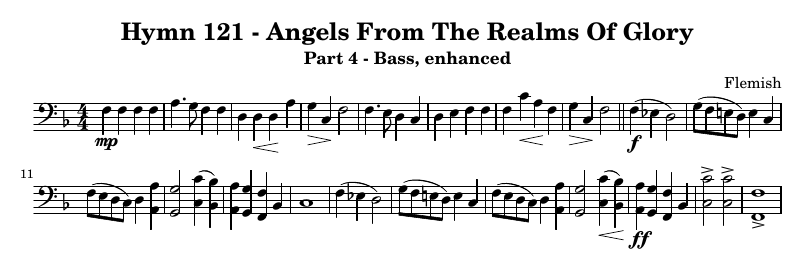
\includegraphics[scale=0.8]{../graphics/Hymn121_BassEnhanced.png}


% -------------------------------------------------------------------------
\section{Using choices in an MFSL script}
% -------------------------------------------------------------------------

Let us go one step further, using \mfslfiles{Hymn121.xml} again, to obtain various scores for a vocal SATB (soprano, alto, tenor, bass) choir.

This example shows the use of a \code{choice} specification and a \code{case} statement, to indicate the various possible score \choice s and what options to use for them, and \code{select} statements or options to the \mfslInterp\ to do the selection.

The actual selection works this way:
\begin{itemize}
\item there can be \code{select} statements at the end of the \script;
\item if such statements are present in the \script, they are used to decide which options to use for the tool;
\item this behaviour can be overridden by the use of \optionNameBoth{select}{sel}, which override the \code{select} statements in the \script if any;
\item if no \code{select} is present in the \script, the default \coiceLabel\ for the \choice\ is implicitly used.
\end{itemize}

The \mfslfiles{Hymn121ForVocalSATBQuartet.mfsl} \script\ contains:
\begin{lstlisting}[language=MFSL]
jacquesmenu@macmini: ~/musicformats-git-dev/mfslfiles > cat Hymn121ForVocalSATBQuartet.mfsl
#!//Users/jacquesmenu/musicformats-git-dev/build/bin/mfsl

###
  This MFSL script contains:
    - a tool specification, telling which MusicFormats tool
      to use, here xml2ly;

    - an input specification, the input source to apply the latter to,
      here file name "Hymn121.xml";

    - a number of MusicFormats options;

    - a SCORE choice specification containing 5 labels,
      each telling which options to use
      to get a score generated with this script and xml2ly/LilyPond;

    - a number of 'select' specifications to choose one or more such SCORE label;

    - an 'every' statement to choose all labels in choice SCORE.
###


# ----------------------------------------------------------
# the MusicFormats tool to be used
# ----------------------------------------------------------

tool : xml2ly ;


# ----------------------------------------------------------
# the input file to be handled by the tool
# ----------------------------------------------------------

input : "Hymn121.xml" ;


# ----------------------------------------------------------
# some commmon options
# ----------------------------------------------------------

# header
  -title "Hymn 121 - Angels From The Realms Of Glory"

# display
#   -display-options-values

# LilyPond
  -lilypond-generation-infos

# dynamics
  -all-wedges-below


# ----------------------------------------------------------
# the labels for the SCORE choice
# ----------------------------------------------------------

# choose names that match the intent
# using uppercase to emphasize a choice name is a matter of taste

choice SCORE :
  tutti |

  soprano | alto | tenor | bass |

  sopranoAndAlto | tenorAndBass,

  default: tutti
;


# ----------------------------------------------------------
# tell which options are to be used depending on SCORE labels
# ----------------------------------------------------------

case SCORE :
	tutti:
	  -output-file-name "Hymn121_SATB_tutti.ly"

    -global-staff-size 17.675

    -subtitle "Tutti"
  ;

	soprano:
	  -output-file-name "Hymn121_SATB_soprano.ly"

    -subtitle '\markup { "B" \hspace #-0.375 \raise #1.5 {\flat} " instruments" }'
    -keep-musicxml-part-id P1

    -msr-rename-part "P1:soprano"

#     -display-lpsr-short
  ;

	alto:
	  -output-file-name "Hymn121_SATB_alto.ly"

    -subtitle "Alto"
    -keep-musicxml-part-id P2
  ;

	tenor:
	  -output-file-name "Hymn121_SATB_tenor.ly"

    -subtitle "Tenor"
    -keep-musicxml-part-id P3

    -global-staff-size 23 # an easier-to-read score is needed
  ;

	bass:
	  -output-file-name "Hymn121_SATB_bass.ly"

    -subtitle "Bass"
    -keep-musicxml-part-id P4

    -ignore-musicxml-lyrics
      # there's a glitch in the last measure of the bass...
  ;

  sopranoAndAlto:
	  -output-file-name "Hymn121_SATB_sopranoAndAlto.ly"

    -subtitle 'Soprano and alto'

    -keep-musicxml-part-id P1
    -msr-rename-part "P1:soprano"
    -lpsr-staff-instrument-name "Voice 1:Soprano"

    -keep-musicxml-part-id P2
    -msr-rename-part "P2:alto"
    -lpsr-staff-instrument-name "Voice 2:Alto"
  ;

  tenorAndBass:
	  -output-file-name "Hymn121_SATB_tenorAndBass.ly"

    -subtitle 'Tenor and bass'

    -keep-musicxml-part-id P3
    -msr-rename-part "P3:tenor"
    -lpsr-staff-instrument-name "Voice 3:Tenor"

    -keep-musicxml-part-id P4
    -msr-rename-part "P4:bass"
    -lpsr-staff-instrument-name "Voice 4:Bass"

    -ignore-musicxml-lyrics
      # there's a glitch in the last measure of the bass...
  ;
;


# ----------------------------------------------------------
# choosing which score(s) to generate
# ----------------------------------------------------------

###
  Comment/uncomment the statements below to choose
  either individual SCORE labels or all of them.
  A group of 'select' statements and an 'every' statement
  are mutually exclusive.

  The 'select' statements choose one particular label each,
  overriding the default "tutti" label setting in the 'choice' statement.

  This can also be done with the 'select' option to the MFSL interpreter such as:
    -select SCORE:tenor -select SCORE:alto

  The 'all' pseudo-label causes all the existing labels for the given choice
  to be selected.

  This can also be done with this option to the MFSL interpreter:
    -select SCORE:all
###

# select SCORE : tutti ;
# select SCORE : soprano ;
# select SCORE : alto ;
# select SCORE : tenor ;
# select SCORE : bass ;

# select SCORE: sopranoAndAlto ;
select SCORE: tenorAndBass ;
\end{lstlisting}


% -------------------------------------------------------------------------
\section{Running the tool for one or more choice labels}
% -------------------------------------------------------------------------

One or more can be selected by \code{select]} statements or with the \optionNameBoth{select}{sel} option.
With:
\begin{lstlisting}[language=MFSL]
select SCORE: tenorAndBass ;
\end{lstlisting}

 or:  %%%JMI
\begin{lstlisting}[language=Terminal]
mfsl
\end{lstlisting}

we get this score:\\
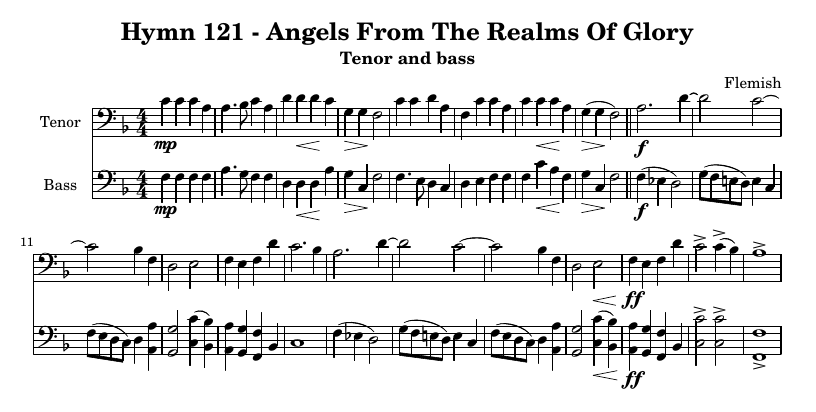
\includegraphics[scale=0.8]{../graphics/Hymn121_SATB_tenorAndBass.png}


% -------------------------------------------------------------------------
\section{Running the tool for all choice labels}
% -------------------------------------------------------------------------

With:
\begin{lstlisting}[language=Terminal]
./Hymn121ForVocalSATBQuartet.mfsl -select SCORE:all
\end{lstlisting}

we get all these \lily\ files:
\begin{lstlisting}[language=TerminalSmall]
jacquesmenu@macmini: ~/musicformats-git-dev/mfslfiles > ls -sal Hymn121_SATB_*.ly
 8 -rw-r--r--@ 1 jacquesmenu  staff   3964 Apr  6 21:39 Hymn121_SATB_alto.ly
 8 -rw-r--r--@ 1 jacquesmenu  staff   3881 Apr  6 21:39 Hymn121_SATB_bass.ly
 8 -rw-r--r--@ 1 jacquesmenu  staff   3931 Apr  6 21:39 Hymn121_SATB_soprano.ly
16 -rw-r--r--@ 1 jacquesmenu  staff   6381 Apr  6 21:39 Hymn121_SATB_sopranoAndAlto.ly
 8 -rw-r--r--@ 1 jacquesmenu  staff   3809 Apr  6 21:39 Hymn121_SATB_tenor.ly
16 -rw-r--r--@ 1 jacquesmenu  staff   6048 Apr  6 21:39 Hymn121_SATB_tenorAndBass.ly
24 -rw-r--r--  1 jacquesmenu  staff  10405 Apr  6 21:39 Hymn121_SATB_tutti.ly
\end{lstlisting}

One of these scores is:\\
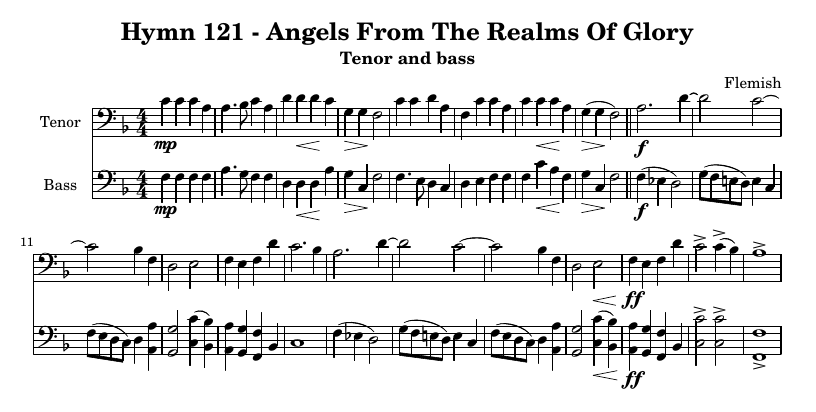
\includegraphics[scale=0.8]{../graphics/Hymn121_SATB_tenorAndBass.png}


% -------------------------------------------------------------------------
\section{Using the MFSL interpreter in shell scripts}\label{Using the MFSL interpreter in shell scripts}
% -------------------------------------------------------------------------

The \mfslInterp\ is a regular executable application, and as such, it can be used in scripts.

This author uses for exemple \mfslfiles{minimal.bash}:
\begin{lstlisting}[language=Terminal]
jacquesmenu@macmini: ~/musicformats-git-dev/mfslfiles > cat minimal.bash
#!/bin/bash

set -x

MINIMAL_LY=Minimal.ly

./minimal.mfsl > ${MINIMAL_LY}

ls -sal ${MINIMAL_LY}

# on Mac OS, 'open' launches the application set by the user
# for a given extension, here '.ly',
# to diplay the file on-screen

open ${MINIMAL_LY}

set +x
\end{lstlisting}

The \code{set} \bash\ commands toggle an echo of the commands on and off.

The trace produced when running this script is:
\begin{lstlisting}[language=Terminal]
jacquesmenu@macmini: ~/musicformats-git-dev/mfslfiles > ./minimal.bash
+ MINIMAL_LY=Minimal.ly
+ ./minimal.mfsl
+ ls -sal Minimal.ly
24 -rw-r--r--@ 1 jacquesmenu  staff  11769 Apr  5 18:24 Minimal.ly
+ open Minimal.ly
+ set +x
\end{lstlisting}


% -------------------------------------------------------------------------
\section{A last MFSL example}
% -------------------------------------------------------------------------

This time, we will create a number of scores for a harmony band, using \lily\ \code{\textbackslash markup} s in MFSL character strings.

The \script\ is \mfslfiles{Hymn121ForHarmonyBand.mfsl}:
\begin{itemize}
\item it contains several \code{case} statements, for readability;
\end{itemize}

\begin{lstlisting}[language=MFSL]
# basic stuff

case SCORE :
	director:
    -global-staff-size 17.675
    -ragged-bottom off
  ;

  part1_C_instruments,
  part2_Bb_instruments,
  part3_Bb_instruments,
  part4_Bb_instruments,
  part4_BassGuitar:
    -ambitus
    -ragged-bottom off
  ;
;
\end{lstlisting}

\begin{lstlisting}[language=MFSL]
# scores appearance

case SCORE :
	director:
    -global-staff-size 17.675
    -ragged-bottom off
  ;

  part1_C_instruments:
  ;

  part2_Bb_instruments:
  ;

  part3_Bb_instruments:
  ;

  part4_Bb_instruments:
  ;

  part4_BassGuitar:
    -ambitus
    -ragged-bottom off
  ;
;
\end{lstlisting}

\begin{lstlisting}[language=MFSL]
# scores identification

case SCORE :
	director:
	  -output-file-name
	    "Hymn121_band_director.ly"
    -subtitle
      "Director - in C"
  ;
 o
# ... ... ...
\end{lstlisting}

\begin{lstlisting}[language=MFSL]
# scores contents

case SCORE :
	director:
    -ignore-musicxml-lyrics
      # there's a glitch in the last measure of the bass...
  ;

	part1_C_instruments:
    -keep-musicxml-part-id P1
    -msr-rename-part "P1:partOne_C_instruments"

    -lpsr-staff-instrument-name "Voice 1:C instruments"
    -indent '3.5\cm'
  ;

	part2_Bb_instruments:
    -keep-musicxml-part-id P2
    -msr-rename-part "P2:partTwo_Bb_instruments"

    -indent '2.5\cm'
    -lpsr-staff-instrument-name
      # let's use LilyPond's '\markup' possibilities
      # successive MFSL character strings are concatenated into a single one
      "Voice 2"
      ":"
      '\markup {'
        '\center-column {'
          '\line { "B" \hspace #-0.375 \raise #1.5 {\flat} }'
          '\line { "instruments" }'
        '}'
      '}'

    -lilypond-transpose-part-id P2=bes
  ;

# ... ... ...
\end{lstlisting}

\mfslfiles{Hymn121ForHarmonyBand.mfsl} can be used to obtain all these \lily\ files:
\begin{lstlisting}[language=TerminalSmall]
jacquesmenu@macmini: ~/musicformats-git-dev/mfslfiles > ls -l Hymn121_harmony_*.ly
-rw-r--r--@ 1 jacquesmenu  staff  9765 Apr  6 18:04 Hymn121_band_director.ly
-rw-r--r--@ 1 jacquesmenu  staff  3366 Apr  6 18:04 Hymn121_band_part1_C_instruments.ly
-rw-r--r--@ 1 jacquesmenu  staff  3627 Apr  6 18:04 Hymn121_band_part2_Bb_instruments.ly
-rw-r--r--  1 jacquesmenu  staff  3444 Apr  6 18:04 Hymn121_band_part3_Bb_instruments.ly
-rw-r--r--@ 1 jacquesmenu  staff  3300 Apr  6 18:04 Hymn121_band_part4_BassGuitar.ly
-rw-r--r--@ 1 jacquesmenu  staff  3454 Apr  6 17:59 Hymn121_band_part4_Bb_instruments.ly
\end{lstlisting}

One of the scores produced by \lily\ is:\\
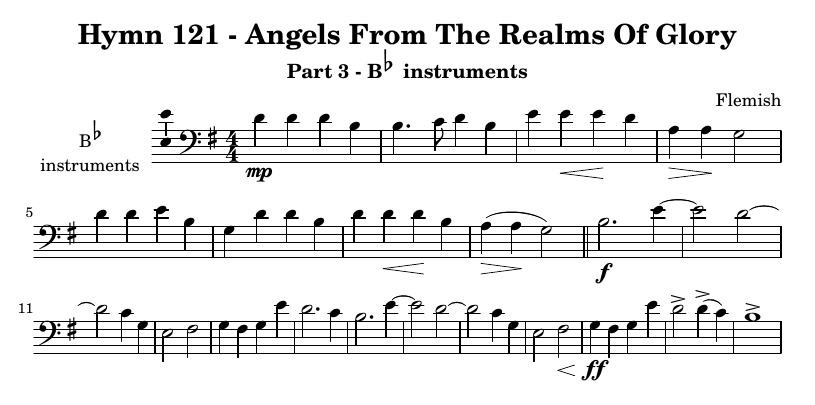
\includegraphics[scale=0.8]{../graphics/Hymn121_band_part3_Bb_instruments.png}


% -------------------------------------------------------------------------
\section{MFSL language details}
% -------------------------------------------------------------------------

To be completed. %%%JMI


%% -------------------------------------------------------------------------
%\section{Error handling in MFSL scripts}
%% -------------------------------------------------------------------------
%
%%%JMI


% -------------------------------------------------------------------------
\section{Behind the scenes\dots}
% -------------------------------------------------------------------------

The \mfslInterp\ is organized as too \pass es:
\begin{enumerate}
\item a first pass analyses the script body and builds an internal representation, which is displayed by the \optionNameBoth{trace-choices}{tchoices} option;

\item the second pass uses the informations thus collected to launch the tool as many times as needed, depending on \code{select}  usage in the script body and the \optionNameBoth{select}{sel} options to the \mfslInterp.
\end{enumerate}
